\section{Cosmological Models}
\subsection{Hubble's constant and the scale factor}

The Hubble's constant can be expressed using the Friedmann equation. We know that the recession velocity $ \vec{v} = \frac{d\vec{r}}{dt} $. Since $ \vec{r}=a\vec{x} $ and $ \vec{x}$ is constant, we get $ \vec{v} = \frac{\dot{a}}{a}\vec{r} $. Hence using Hubble's law, we can say that $ H=\frac{\dot{a}}{a} $. Hence the term H can be substituted in Friedmann equation to obtain:

\begin{equation}
    H^2 = \frac{8{\pi}G}{3}\rho - \frac{k}{a^2}
\end{equation}

Furthermore, the relation between wavelength of observed light and the scale factor can be obtained using Hubble's law. The relative velocity between two nearby objects, such as galaxies is gievn by $dv = Hdr = \frac{\dot{a}}{a}r$. Since the objects are assumed to be nearby, we can say that $d\lambda = \lambda_{r}-\lambda_{e}$ (wavelength received - wavelength emitted). According to Doppler's law , $\frac{d\lambda}{\lambda_{e}} = \frac{dv}{c}$.Since the wavelength gets redshifted when emitting object moves farther away, ${d\lambda}$ is positive.

\begin{center}
\begin{math}
    \frac{d\lambda}{\lambda_{e}} = \frac{\dot{a}}{a}\frac{dr}{c} = \frac{\dot{a}}{a}dt = \frac{da}{a}
\end{math}
\end{center}


\begin{center}
    $\implies{\lambda \propto a}$
\end{center}

The increase in wavelength can also be thought of as wavelength getting "stretched" due to the expansion of space. The redshift, z, is defined as :

\begin{center}
    $1+z = \frac{\lambda_{r}}{\lambda_{e}} = \frac{a(t_r)}{a(t_e}$
\end{center}

\subsection{Solutions to Friedmann Equation}
In order to solve the Friedmann equation, we need information about the pressure and density of the universe, which will be described by an equation called equation of state. 

The universe is believed to consist of matter and radiation. Matter refers to non-relativistic material in cosmology while radiation includes all relativistic particles (typically photons and neutrinos). Matter has negligible pressure ($p = 0$) and radiation has a pressure given by $p = \frac{{\rho}c^2}{3}$.

The Friedmann equation has a crucial element of symmetry; the scale factor always appears as a fraction ${\dot{a}}{a}$, which means that it can be scaled according to our convenience. Hence we take the value of a at present time to be 1. The value of $k$ is assumed to be \textbf{zero} in this analysis. 

\begin{itemize}
    \item Case 1: Matter: \\
    Taking p to be 0 in the fluid equation gives the following:
    \begin{center}
    \begin{math}
         \dot{\rho} + 3\frac{\dot{a}}{a}{\rho} = 0 \implies \ln(\rho) = -3\ln{a} + const \implies \rho \propto \frac{1}{a^3}
    \end{math}
    \end{center}
    In cosmology, the present value of parameters is usually represented by a subscript. Hence, 
    ${\rho}=\frac{{\rho}_0}{a^3}$. Substituting this in the Friedmann equation gives ${\dot{a}^2} = \frac{8{\pi}G{\rho_{0}}}{3}\frac{1}{a}$.
    This equation can further be solved, from which we obtain a power law solution $a(t)=(\frac{t}{t_0})^{\frac{2}{3}}$ and $H=\frac{2}{3t}$.
    \item Case 2: Radiation: \\
    The presence of radiation pressure $p = \frac{{\rho}c^2}{3}$ changes the fluid equation from the matter dominated case and leads to the following:
    \begin{center}
    \begin{math}
         \dot{\rho} + 4\frac{\dot{a}}{a}{\rho}=0 \implies \rho \propto \frac{1}{a^4}
    \end{math}
    \end{center}
    This is again substituted in the Friedmann equation and another power law solution is obtained. a(t) = $(\frac{t}{t_0})^{\frac{1}{2}}$
    \item Case 3: Mixtures: \\
    When both matter and radiation are present, which is what is expected in our universe, the total density $\rho$ is given as sum of densities of matter and radiation components. Obtaining $\rho$ as a function of time is not simple when $\rho_{mat}$ and $\rho_{rad}$ have approximately equal contributions to total density, but can be analysed when one dominates over the other. In both cases we obtain that matter domination is more stable as matter density falls slower compared to radiation density. Hence the universe would eventually end up being dominated by matter in its later stages.
\end{itemize}

\begin{figure}[H]
    \centering
    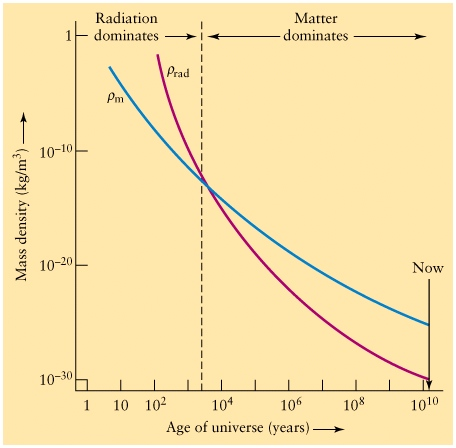
\includegraphics[width=0.6\textwidth]{figure 2.jpg}
    \caption{This plot shows how the density contribution from matter and radiation changes over time. It can be seen that the Universe starts out being dominated by radiation, which then shifts to matter, due to reasons cited earlier.}
    \label{fig:geometry}
\end{figure}

The way the universe evolves can change depending on the value of $k$ as well. Since the expansion of the universe is governed by the scale factor a and rate of expansion by $\dot{a}$, the Hubble factor, being a ratio of the two, is a good measure of expansion. The universe will stop expanding when H=0. 

Hence it is evident that H cannot be zero when k is negative or 0. In fact when k is negative the density factor becomes negligible compared to the $k$ term, leading to $a \propto t$. This is known as \textbf{free expansion} as the velocity of expansion is 0.

When $k>0$, H must become 0 at one point in time since the $k$ term will become large enough to cancel out the density term. Hence re-collapse of the universe will happen in closed geometries.

\subsection{Observational Parameters}
Since the Friedmann equation isn't constant in time, certain factors such as present expansion rate, present density etc. need to be fixed by observation. 

The first parameter is the Hubble constant $H_0$, which is also the expansion rate of the universe. It can be calculated using Hubble's law if velocity and distance of astronomical objects are known. Velocities are obtained from redshift measurements, but this measured velocity also has a component of velocity corresponding to the relative motion of objects (called \textbf{peculiar velocity}), in addition to the universe's rate. This issue is overcome by measuring velocities if object which are very far away, since cosmological principle demands that the peculiar velocity be independent of the scale of the universe. Distance measurement using standard candles, such as Cepheid variables or supernovae enables us to calculate $H_0$. State of the art measurements have calculated it to a good accuracy, giving $H_0=100h$ $kms^{-1} Mpc^{-1}$, where $h=0.72\pm0.08$ is an uncertainty factor. \\

The second parameter is the density parameter. From the equation $H^2 = \frac{8{\pi}G}{3}\rho - \frac{k}{a^2}$, we can see that for a given H, there exists a corresponding value of $\rho$ such that $k$ goes to zero. This density is knows as the critical density:

\begin{equation}
    \rho_{c}(t) = \frac{3H^2}{8{\pi}G}
\end{equation}

$\rho_{c}$ changes with time due to its dependence on H. Plugging in the present value of the Hubble's constant gives the value of critical density to be $1.88h^2$ x $10^{-26}$ $kgm^{-3}$, which is a very small value of density compared to objects in everyday life. However, when it is expressed in units of $[Solar Mass][Mpc]^{-3}$, its value is of the order of $10^11$. Eventhough the universe may not be flat, the critical density sets a good scale for comparison. Hence the \textbf{density parameter}, $\Omega$ is defined as 

\begin{center}
    $\Omega(t) = \frac{\rho}{\rho_c}$
\end{center}

$\rho$ can be substituted back in the Friedmann equation as $\Omega\rho_c$:

\begin{center}
\begin{math}
  H^2 = \frac{8{\pi}G}{3}{\rho_c}\Omega - \frac{k}{a^2} = H^2\Omega - \frac{k}{a^2}
\end{math}
\end{center} 

\begin{center}
    $\implies \Omega = 1 + \frac{k}{a^2H^2}$
\end{center}

Hence we can see that $k=0$ when $\Omega = 1$

A density parameter corresponding to $k$ can also be defined as $\Omega_k = -\frac{k}{a^2H^2}$, which implies that $\Omega+\Omega_k=1$ \\

The final observation parameter, which is dependent on the above two, is called the \textbf{deceleration parameter}. It can be obtained as follows: 

\begin{center}
\begin{math}
    a(t) = a(t_0) + \dot{a}(t_0)[t-t_0] + \frac{1}{2}\ddot{a}(t_0)[t-t_0]^{2}...
\end{math}
\end{center}

\begin{center}
\begin{math}
   \implies \frac{a(t)}{a(t_0)} = 1+ H_0[t-t_0] - \frac{q_0}{2}H_0^2[t-t_0]^2 + ...
\end{math}
\end{center}

This defines the deceleration parameter $q_0$ as $q_0 = \frac{\ddot{a}(t_0)}{a(t_0}\frac{1}{H_0^2}$. Since $q_0 \propto \ddot{a}(t_0)$, higher its value, faster will be the deceleration. In case of matter dominated universe, $q_0 = \frac{\Omega_0}{2}$. Since $q_0$ is easier to measure, we can obtain values of other parameters from it. Recent observation have shown that $q_0<0$, which means that our universe is accelerating, which is not possible in the models defined earlier. To correct this another parameter was introduced in the Friedmann equation called the \textbf{cosmological constant}.